In this section, we show empirical results of our algorithm on different transferring situations on two datasets: AwA\footnote{The features of AwA dataset is available from http://attributes.kyb.tuebingen.mpg.de/} \cite{lampert2009learning} and Caltech-256\footnote{Images for Caltech-256 is available from http://www.vision.caltech.edu/Image\_Datasets/Caltech256/} \cite{griffin2007caltech}. In real world applications, there are three situations when we transfer the knowledge from one image database to another. Two extreme situations consist in transferring knowledge from either highly related source task (positive transfer), or unrelated source task (negative transfer). The third and the most common one is the intermediate (mixed) case where only some of categories in the source are related and helpful. We design three sets of experiment, called positive, negative and mixed transfer experiment respectively, based on these 3 situations, comparing our algorithm with the baselines to show its effectiveness.
\subsection{Dataset}
Caltch-256 contains 30,607 images from 256 categories. We select the following 10 categories: \textit{bat, bear, dolphin, giraffe, gorilla, horse, leopard, raccoon, skunk, zebra}, containing 1387 images, as our dataset.

AwA dataset consists of 50 animal categories. Its source images is not publicly accessible and we can only access the six pre-extracted feature representations for each image. This property makes it natural as the unknown distribution source dataset to train the prior knowledge. We choose the identical 10 categories as those in Caltech-256 from it, containing 6917 images.

\subsection{Baselines and algorithmic setup}
We compare our algorithm with two kinds of baselines. The first one is methods without leveraging any prior knowledge (no transfer baselines). The second consists of some methods with transfer techniques. Here are the no transfer baselines.

\textbf{No transfer:} LS-SVM trained only on target data. Any transfer algorithm that performs worse than it suffers from negative transfer.

\textbf{Batch:} We combined the source and target data, assuming that we have fully access to all data, to train the LS-SVM. The result of this baseline might be considered as the best performance achieved when the source and target tasks are related. We only perform this baseline in positive transfer experiment, because in the other experiments, its results can't provide any useful information for us.

\textbf{Source+1:} This method only train a new binary LS-SVM for the new category. For the rest of the classes, we use the predictions of the classifiers trained from source data directly. This is arguably the easiest way for transfer learning. The performance of this method can be an indicator whether the data of the source and target task are drawn from similar distribution.

We select the following 3 methods as our transfer baselines. The general property of these 3 methods is that they all try to leverage multiple prior knowledge to benefit the transfer procedure with LS-SVM.

\textbf{MKTL \cite{jie2011multiclass}:} This method uses the output of source models as extra feature inputs, and automatically determine from which source models to transfer and how much to transfer.


\textbf{MULTI-KT \cite{tommasi2014learning}:} This method has similar idea with MKTL. It uses LOO error to determine how much to transfer from source models and convert it into solving the convex optimization problem.

\textbf{MULTIpLE \cite{kuzborskij2013n}:} The basic setting of this method is similar like ours. It is designed to balance the performance between learning the new category and preserving the model from prior knowledge.

For all the experiments in this section, we adopt the same strategy as \cite{kuzborskij2013n} and \cite{tommasi2014learning}, using kernel averaging \cite{gehler2009feature} to compute the average of RBF kernels over the available features on RBF hyperparameter $\{2^{-5},2^{-4},...,2^8\}$. The penalty parameter $C$ is tuned via cross-validation on $\{10^{-5},10^{-4},...,10^8\}$ and the optimal value is reused for all the algorithms.
Two transfer regularization parameters $\lambda1$ and $\lambda2$ are also set via cross-validation on $\{10^{-3},10^{-2},...,10\}$ respectively.

\subsection{Positive transfer: transferring from related sources}
In the extreme case, where the knowledge of the source task is related to the target one, the data of these two tasks can be drawn from the same distribution. 
We perform tow experiments under this setting on both AwA and Caltech. For each dataset, we split the data into two sets. One is treated as the source dataset to train the source model and another is treated as the target dataset for training and testing. We iteratively choose one category as the new category and run the experiment 10 times to get the average performance of each algorithm. The results of the two experiments are reported in Table \ref{tab:C2C} and Table \ref{tab:A2A}. From the results we can see that, in Caltech experiment, our algorithm consistently outperforms all the baselines (even better than Batch method). In AwA dataset, Source+1 outperforms SMITLe when the training size is 5. As we increase the training size, the accuracy of SMITLe increases and outperforms Source+1.

To illustrate the detail performance of our algorithm, we select the experiment result on AwA dataset where horse is chosen as the new category for further explanation. In Figure \ref{fig:awa-a}, we show the average performances of different methods on different training size for 10 experiments. We can observe that, as the training size increases, our method can even outperforms the batch method.
In Figure \ref{fig:awa-b} we provide values of $\gamma$ and $\beta$ compared with the parameters of the runner-up transfer algorithm MULTIpLE. We can see that for transfer knowledge between identical categories, MULTIpLE fixes the transfer parameter ($\gamma$) to be 1 while our method sets greater weights for related prior knowledge. By exploiting the positive prior knowledge more aggressively, SMITLe is able to leverage the prior knowledge and outperforms other methods. For the transfer parameter $\beta$ we can see that MULTIpLE tends to keep $\beta$ greater than 0 and SMITLe works more intuitively, setting positive weight for related categories(giraffe, zebra and bear etc.) and small or even negative weight for unrelated categories (bat, dolphin and skunk etc.).


\begin{figure*}
\centering
\subfloat[Overall accuracy comparision with different baselines. ]{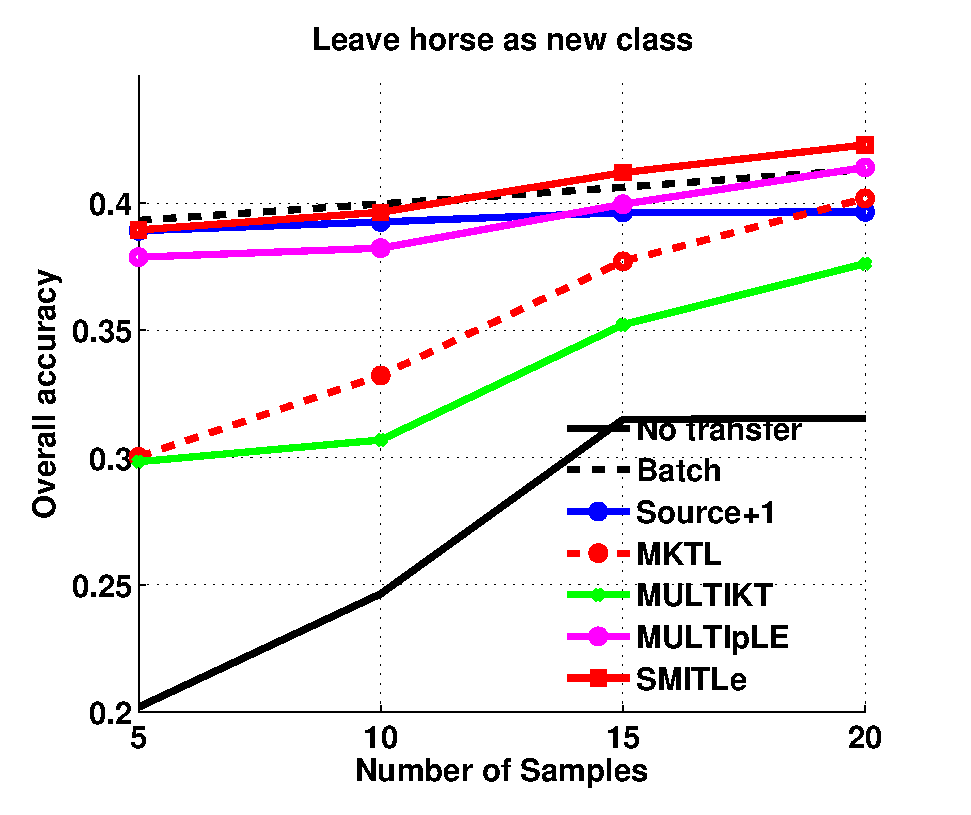
\includegraphics[scale=.4]{fig/A2A_horse.eps}\label{fig:awa-a}}
\subfloat[Comparision with MULTIpLE.] {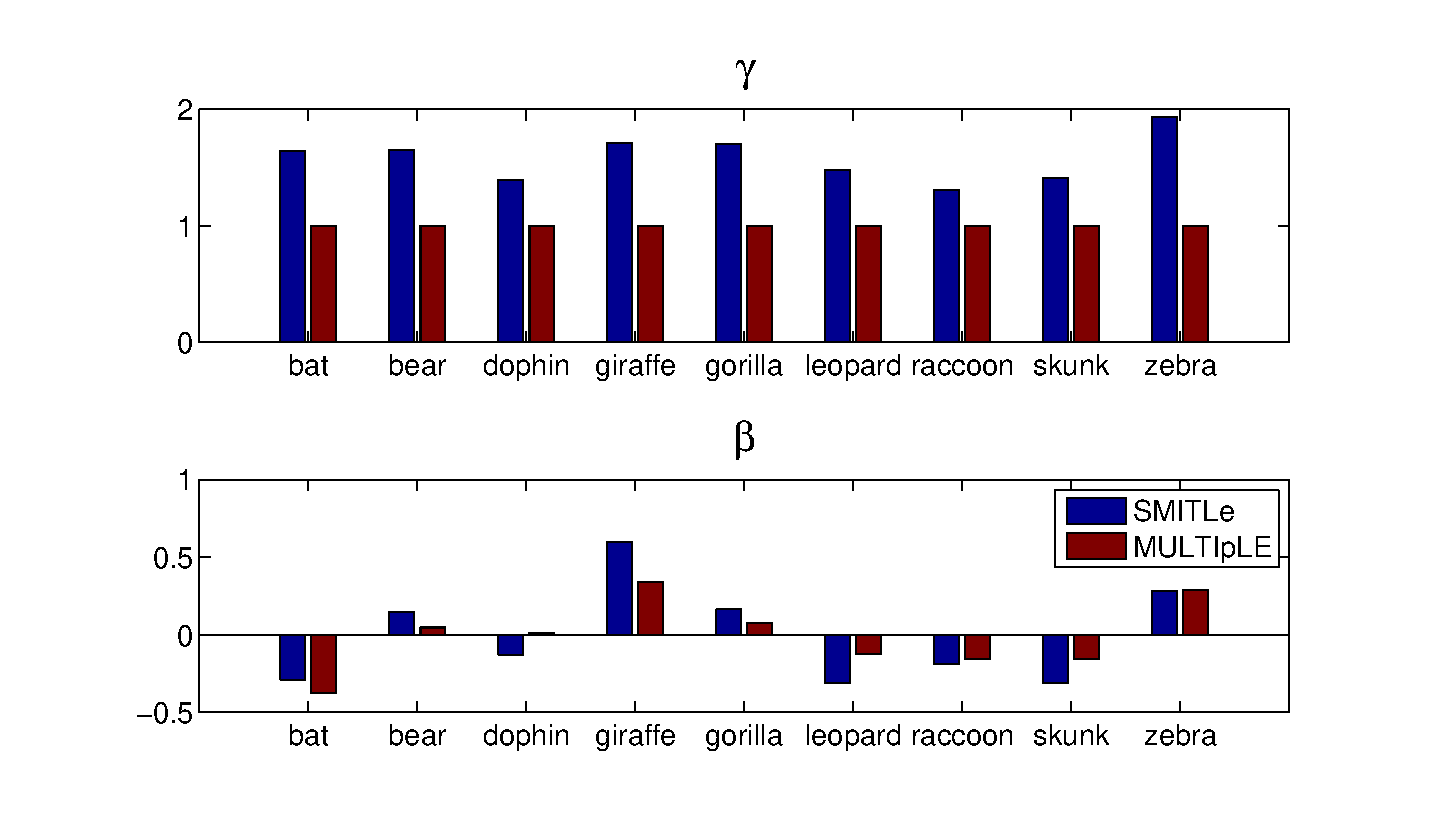
\includegraphics[scale=0.4]{fig/A2A_gama.eps}\label{fig:awa-b}}

\caption{Experiment results for 10 classes, AwA. Horse is used as the new category. From \protect\subref{fig:awa-b} we can see that SMITLe tends to more aggressively exploit the related prior knowledge.}
\label{fig:awa}
\end{figure*}


\begin{table}[htbp]
  \centering
  \caption{Average accuracy in percentage across all categories from Caltech to Caltech with different size of training set in target problem. 30 examples are randomly chosen from each class to train the source classifier and 30 examples from each class are chosen for test. }
    \begin{tabular}{ccccc}
    \toprule
      size per category    & 5     & 10    & 15    & 20 \\
    \midrule
    No transfer &         27.33  &         31.53  &         35.73  &         38.47  \\
    Source+1    &         43.33  &         43.87   &         44.33  &         44.57   \\
    MKTL        &         38.89  &         43.27   &         45.72  &         47.44   \\
    MULTIKT     &         37.96  &         42.89   &         45.96  &         47.32  \\
    MULTIpLE    &         42.63  &         45.63   &         47.81  &         48.73 \\
    SMITLe        &         \textbf{43.53 }&         \textbf{46.45 } &         \textbf{48.25 } &         \textbf{49.15 } \\
        \midrule
    Batch       &         43.77  &         44.73   &         46.67  &         48.00 \\
    \bottomrule
    \end{tabular}%
  \label{tab:C2C}%
\end{table}%

% Table generated by Excel2LaTeX from sheet 'Sheet1'
\begin{table}[htbp]
  \centering
  \caption{Average accuracy in percentage across all categories from AwA to AwA with different size of training set in target problem. 50 examples are randomly chosen from each class to train the source classifier and 200 examples from each class are chosen for test.}
    \begin{tabular}{ccccc}
    \toprule
     size per category    & 5     & 10    & 15    & 20 \\
    \midrule
    No transfer &         23.52  &         26.79  &         29.60  &         31.50  \\
    Source+1    &         \textbf{ 39.00 } &         \textbf{ 39.34 } &         39.62 &         39.74  \\
    MKTL        &         31.46  &         34.76  &         37.41  &         38.81  \\
    MULTIKT     &         29.86  &         32.86  &         35.22  &         36.33  \\
    MULTIpLE    &         37.80  &         38.81  &         39.80  &         40.47  \\
    SMITLe        &        37.83  &         { 39.31 } &         \textbf{ 40.37 } &         \textbf{41.09} \\
        \midrule
    Batch       &         39.62  &         40.18  &         40.67  &         41.44  \\
    \bottomrule
    \end{tabular}%
  \label{tab:A2A}%
\end{table}%



\subsection{Negative transfer: transferring from unrelated sources}
In this section, we show how our method performs in transferring knowledge between two different datasets, from AwA dataset to Caltech dataset. Following the settings in previous experiment, the source models are trained from AwA dataset and transfered to Caltech dataset. We iteratively select one category as the new one, running multiple times to get the average results for all the algorithms. We show the average performance of each algorithm in Table \ref{tab:A2C}. We can see that negative transfer does happen when transferring the knowledge from AwA to Caltech for all the algorithms except for ours. From the performance of Source+1, we can see that applying the source models directly leads to poor performance. We can conclude that even though these two datasets share some categories, the data distribution of the feature representation for the same category is not consistent. 

Still we take the experiment where horse is considered as the new category to see the detail performance of each algorithm and show the it in Figure \ref{fig:awa} . From here we can see that, not surprisingly, the accuracy of SMITLe shows similar accuracy to the no transfer baseline, while other methods suffer from negative transfer and perform even worse than no transfer baseline. In Figure \ref{fig:awa-b} we show the parameters learned for each classes in SMITLe in comparison with MULTIpLE. We can see that, when the prior knowledge is unrelated, SMITLe resists utilizing the prior knowledge and therefore shows almost identical accuracy to the no transfer baseline.
%\begin{figure*}
%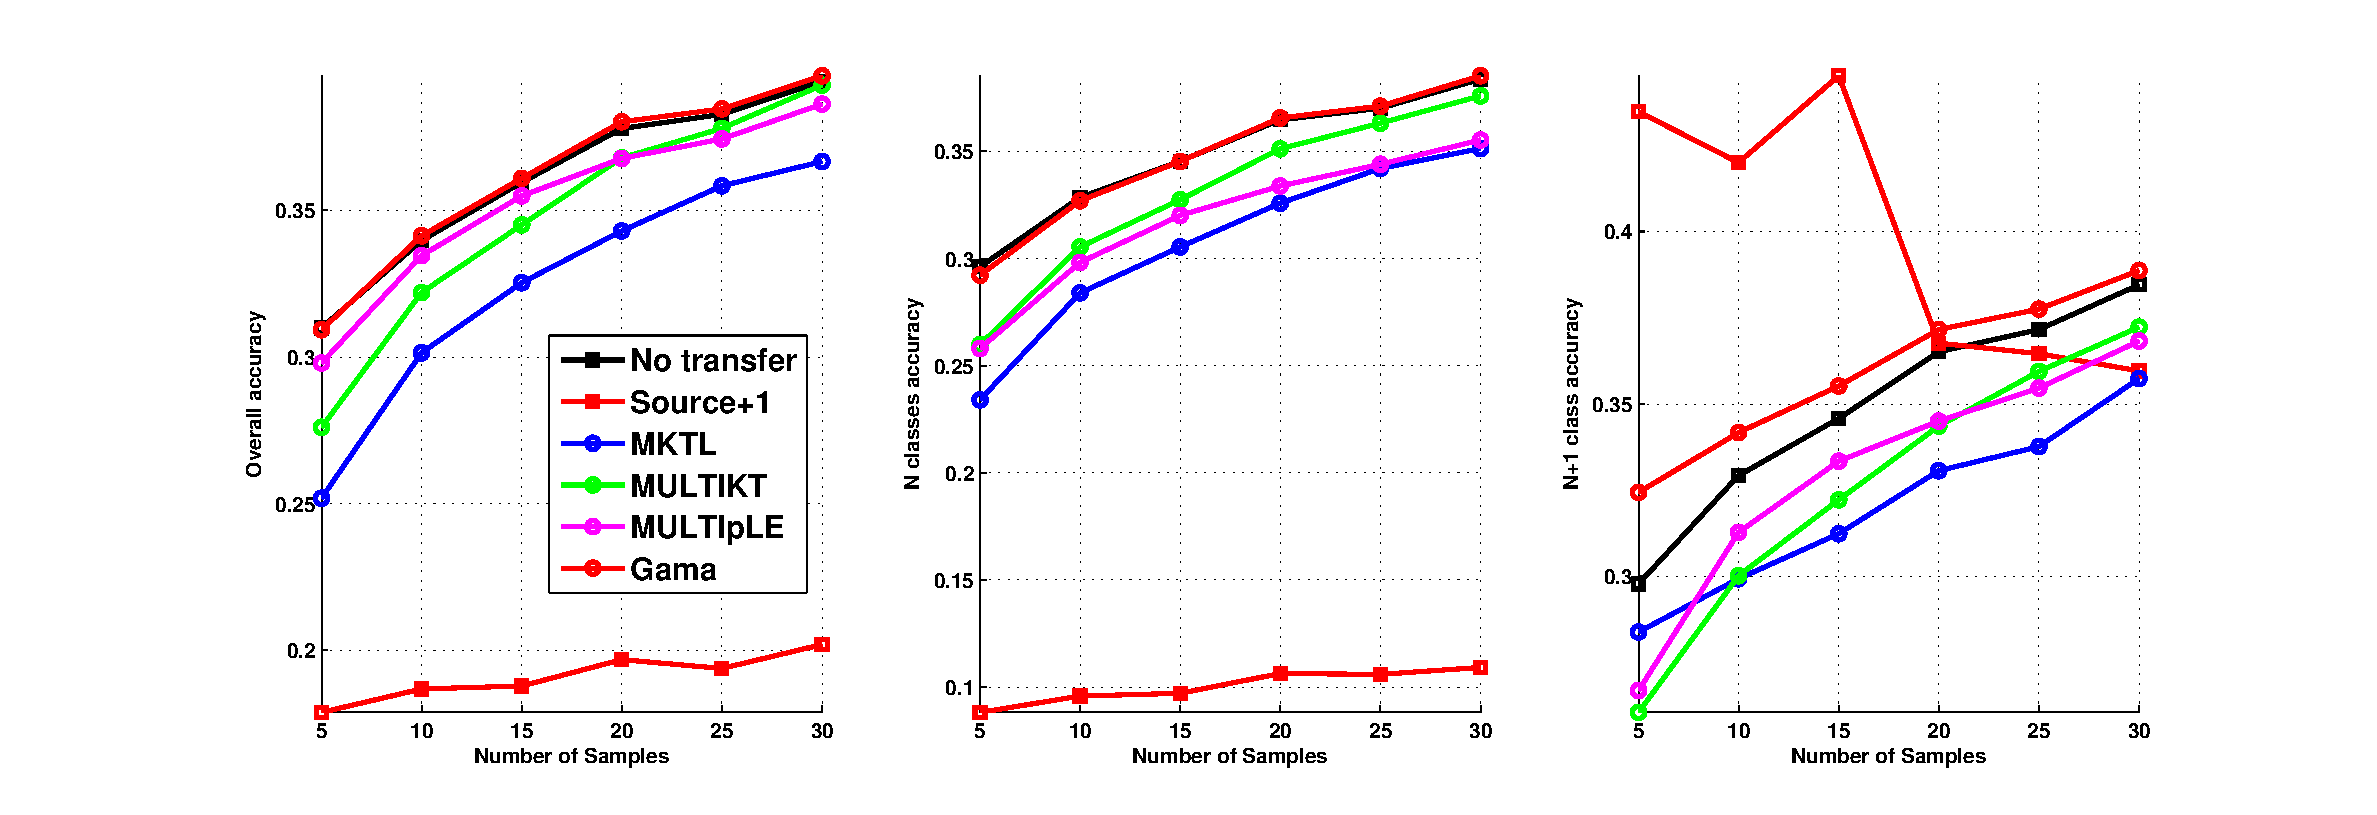
\includegraphics[width=\textwidth,height=5cm]{fig/A2C_RBF_PHOG.eps}
%\caption{Transferring from AwA to Caltech-256.}
%\end{figure*}
% Table generated by Excel2LaTeX from sheet 'Sheet1'

\begin{figure*}
	\centering
	\subfloat[Overall accuracy in percentage comparision with different baselines. ]{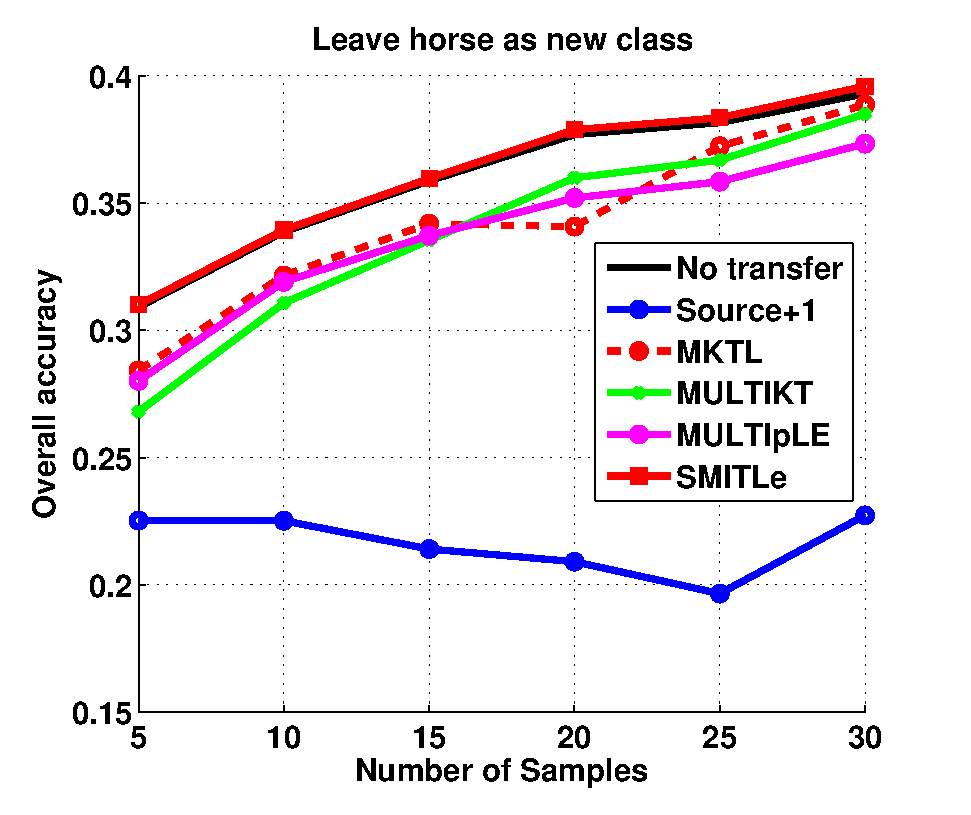
\includegraphics[scale=.4]{fig/A2C_horse.eps}\label{fig:a2c-a}}
	\subfloat[Comparision with MULTIpLE.] {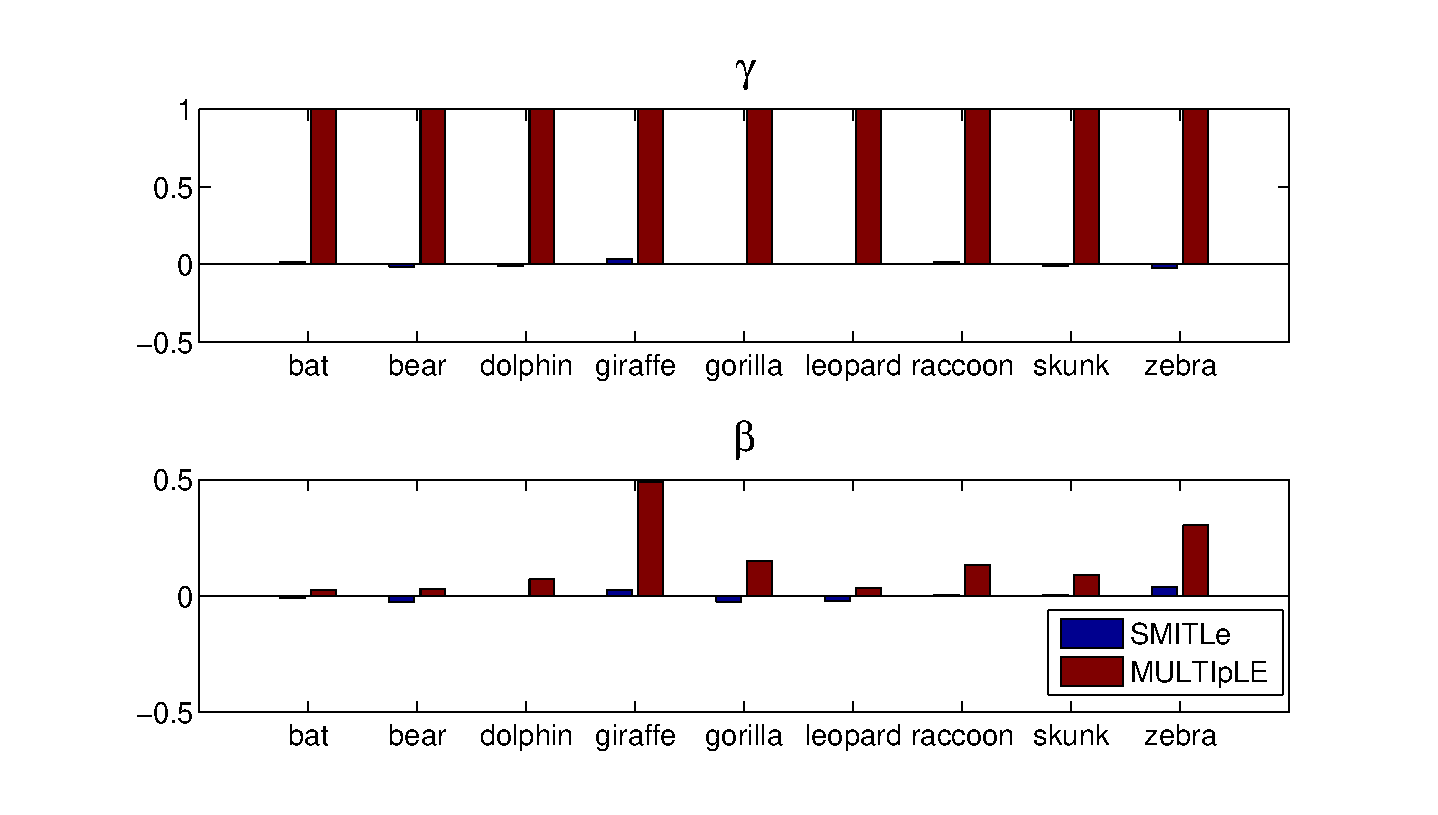
\includegraphics[scale=0.4]{fig/A2C_gama.eps}\label{fig:a2c-b}}
	\caption{Experiment results for 10 classes, AwA. Horse is used as the new category.}
	\label{fig:a2c}
\end{figure*}


\begin{table}[htbp]
  \centering
  \caption{Average accuracy in percentage across all categories from AwA to Caltech. Examples in AwA are used to train prior models. Different number of training size is randomly selected from Caltech dataset.}
    \begin{tabular}{ccccccc}
    \toprule
                & 5              & 10             & 15             & 20             & 25             & 30 \\
    \midrule
    No transfer &         \textbf{ 30.99 } &         33.97  &         35.95 &         37.78  &         38.27  &         39.39  \\
    Source+1    &         17.89  &         18.69  &         18.79  &         19.69  &         19.39  &         20.20  \\
    MKTL        &         25.19  &         30.14  &         32.53  &         34.30  &         35.83  &         36.66  \\
    MULTIKT     &         27.60  &         32.19  &         34.51  &         36.78  &         37.79  &         39.27  \\
    MULTIpLE    &         29.79  &         33.45  &         35.49  &         36.77  &         37.43  &         38.62  \\
    SMITLe        &       30.93  &         \textbf{ 34.13 } &         \textbf{  36.09 } &         \textbf{38.01} &         \textbf{38.46} &         \textbf{39.59} \\
    \bottomrule
    \end{tabular}%
  \label{tab:A2C}%
\end{table}%

\subsection{Transferring from mixed sources}
In real applications, extreme situation is rare. For most multi-source transfer learning tasks, there should always be some related and useful sources as well as some unrelated ones. In this part, we show how SMITLe performs in the mixed sources.

From negative transfer experiments we see that the knowledge from AwA is unrelated to Caltech and vice versa. To generate mixed sources, we follow the settings in our positive transfer experiment, splitting the AwA dataset into two datasets, and replace the data of some categories in the source dataset with the data from Caltech. 
For example, if bat is considered as the new category and we have to replace 3 categories, we choose the data from 3 out of 9 categories (10 categories except for bat) in Caltech to replace the the source data accordingly. 

We show the performances across all categories of different algorithms in Figure \ref{fig:a2a_bad_3} and Figure \ref{fig:a2a_bad_4} where 3 and 4 categories in the source data are replaced by the data from Caltech respectively. From the figures we can see that in almost every case, SMITLe shows improved or equivalent performance than other baselines. Unfortunately, we fail to get intuitive interpretation for $\gamma$ and $\beta$ as we showed in previous experiments. The improved performance of SMITLe could be due to the loss function we designed. Compared to other transfer baselines, the loss function Eq. \eqref{eq:loss} is able to control the transfer parameters $\gamma$ and $\beta$ to prevent negative transfer. For other transfer baselines , such as Multi-KT and MULTIpLE, they try to optimize the multi-class prediction loss directly with non-negative L2 ball constraint, which could not be able to handle the negative transfer effectively.


\begin{figure*}
  \centering
  \subfloat[]{    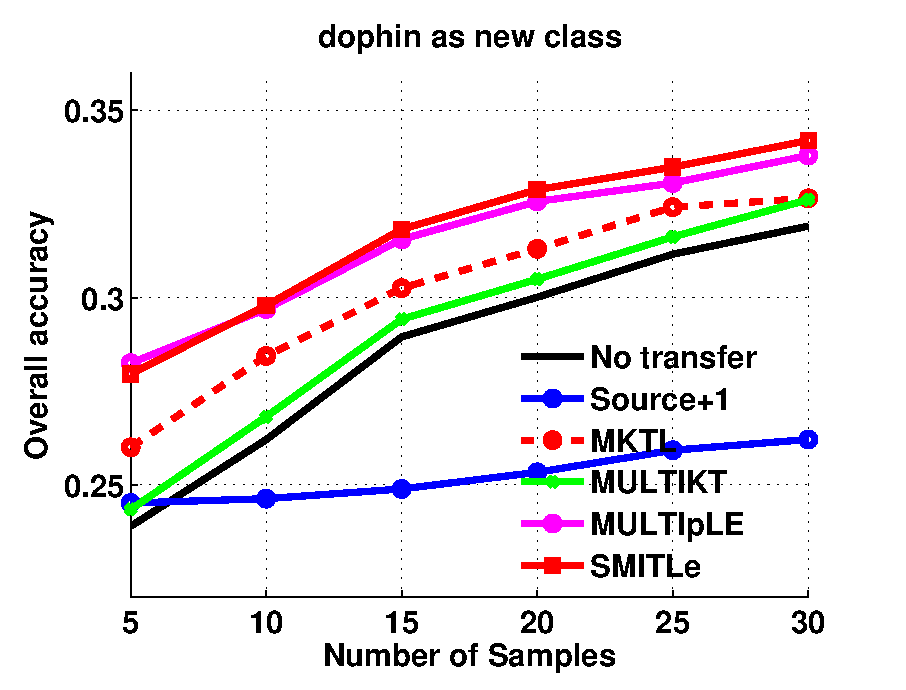
\includegraphics[width=0.18\textwidth]{fig/A2A_bad/A2A_bad_3c_3.eps}  }
  \subfloat[]{    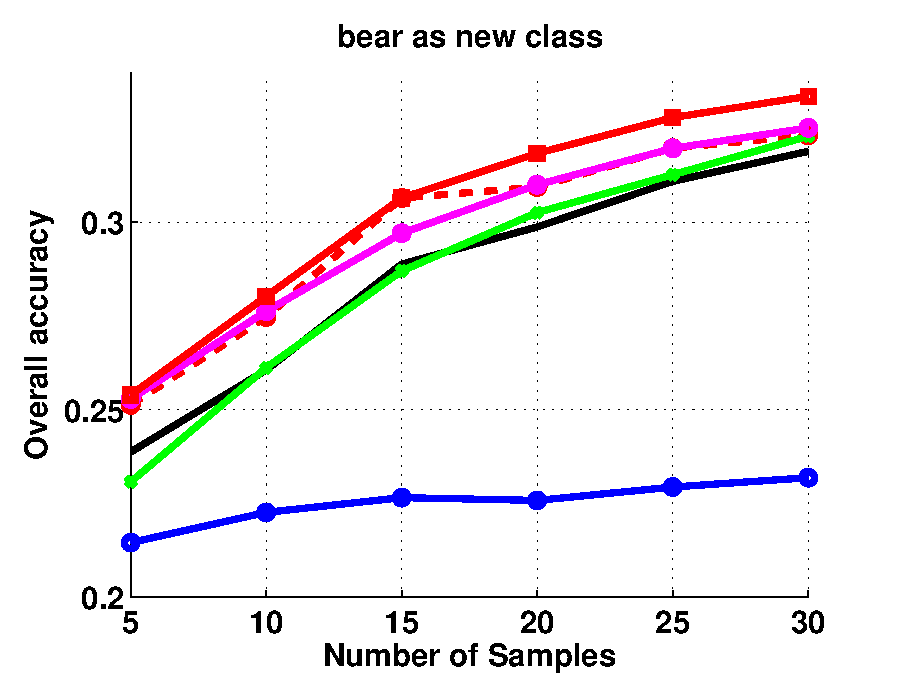
\includegraphics[width=0.18\textwidth]{fig/A2A_bad/A2A_bad_3c_2.eps}  }
  \subfloat[]{    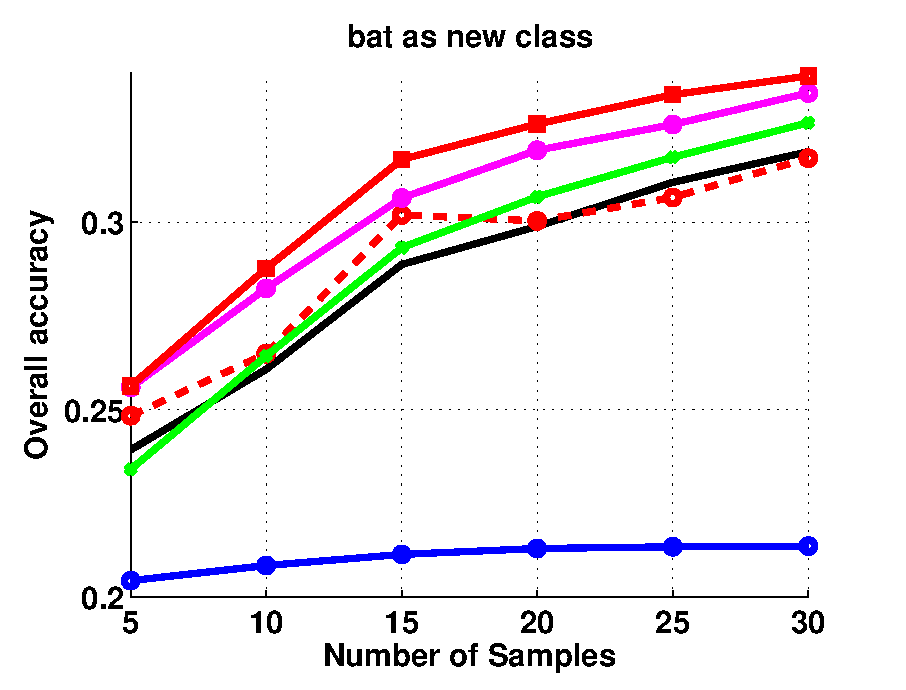
\includegraphics[width=0.18\textwidth]{fig/A2A_bad/A2A_bad_3c_1.eps}  }
  \subfloat[]{    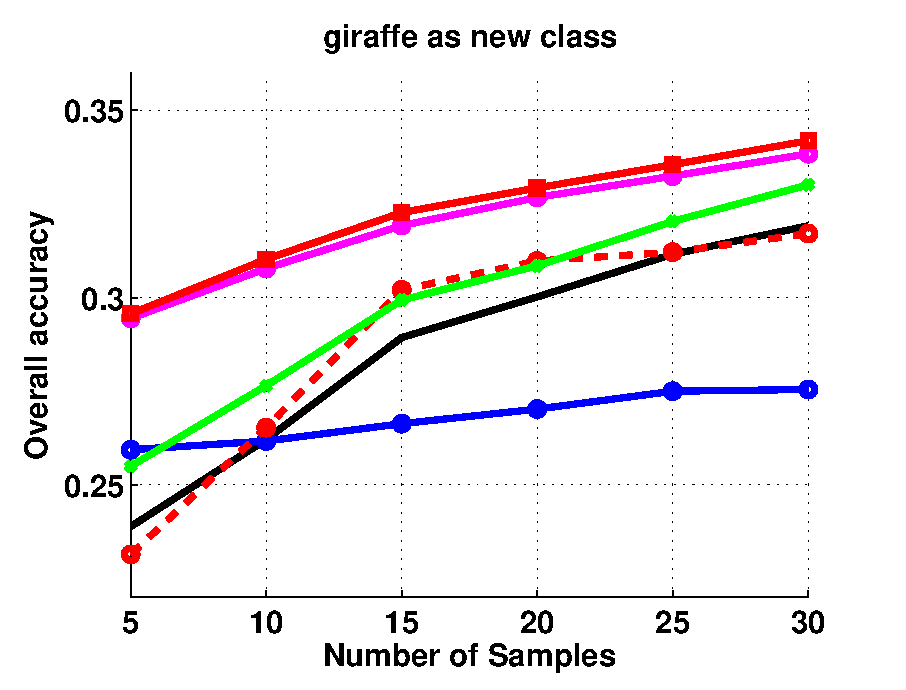
\includegraphics[width=0.18\textwidth]{fig/A2A_bad/A2A_bad_3c_4.eps}  }
  \subfloat[]{    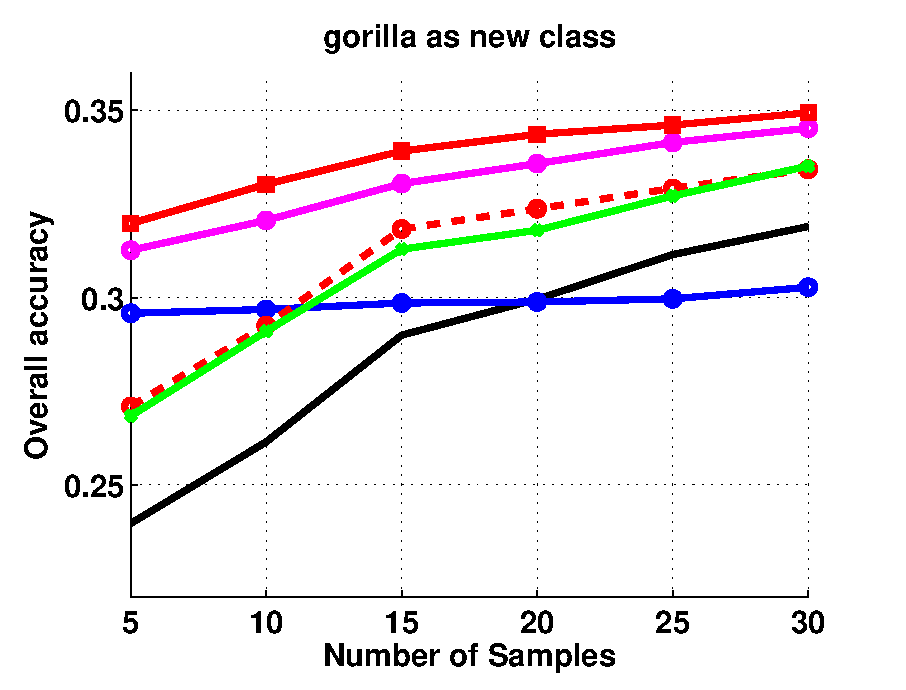
\includegraphics[width=0.18\textwidth]{fig/A2A_bad/A2A_bad_3c_5.eps}  }\\
  \subfloat[]{    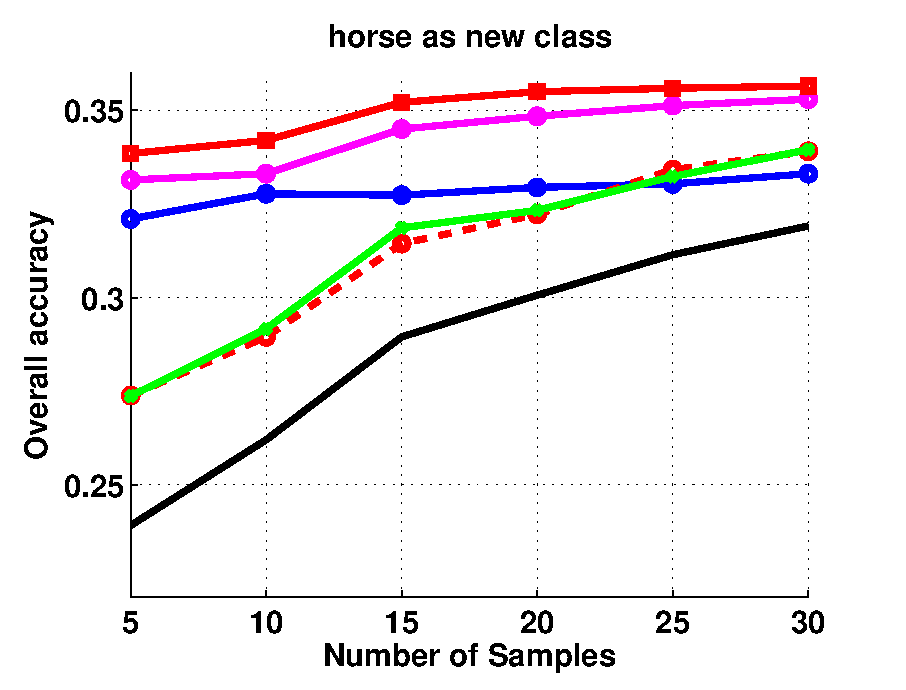
\includegraphics[width=0.18\textwidth]{fig/A2A_bad/A2A_bad_3c_6.eps}  }
  \subfloat[]{    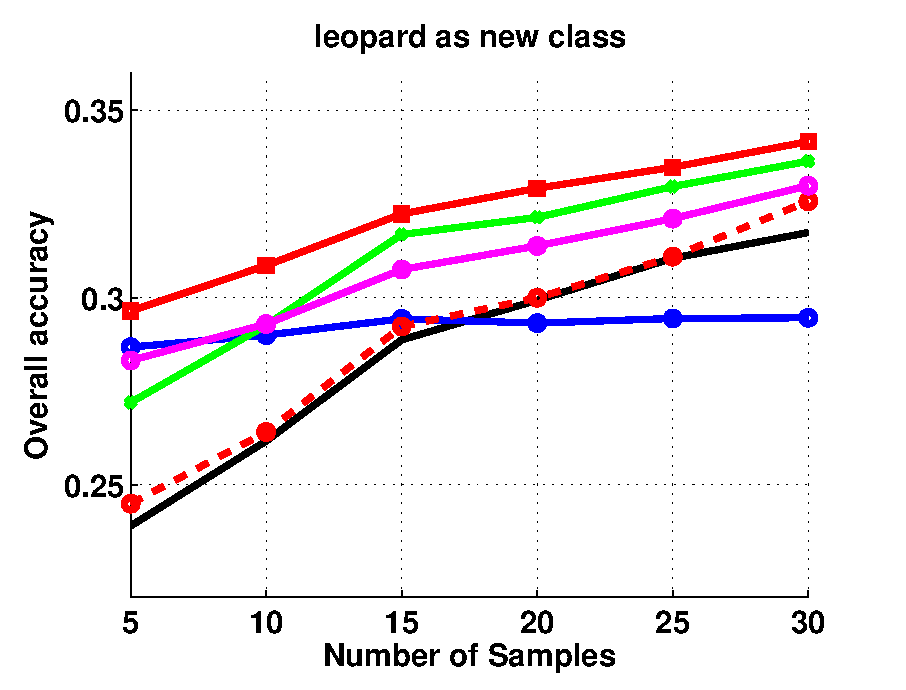
\includegraphics[width=0.18\textwidth]{fig/A2A_bad/A2A_bad_3c_7.eps}  }
  \subfloat[]{    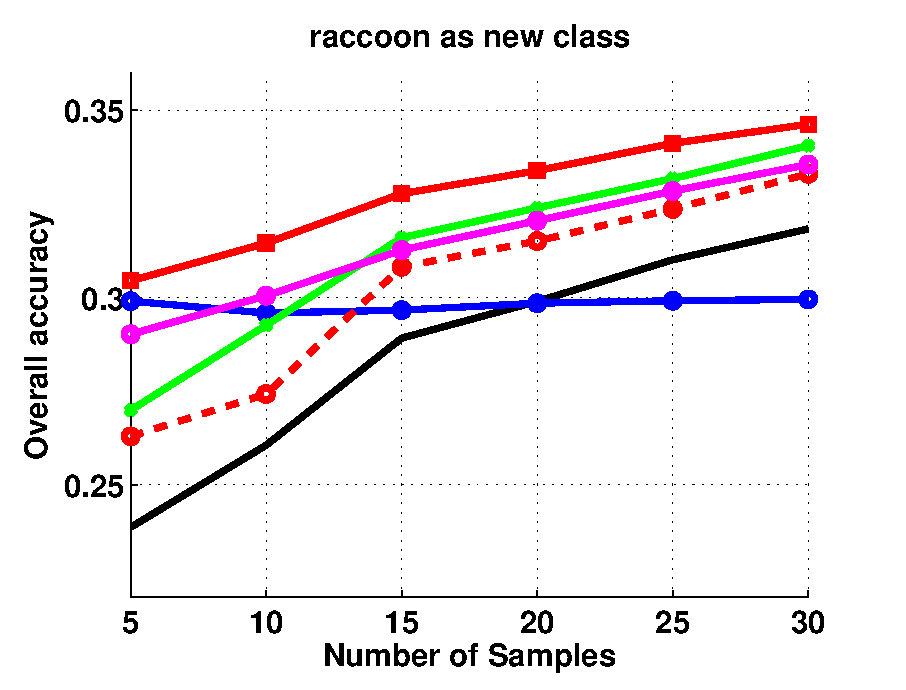
\includegraphics[width=0.18\textwidth]{fig/A2A_bad/A2A_bad_3c_8.eps}  }
  \subfloat[]{    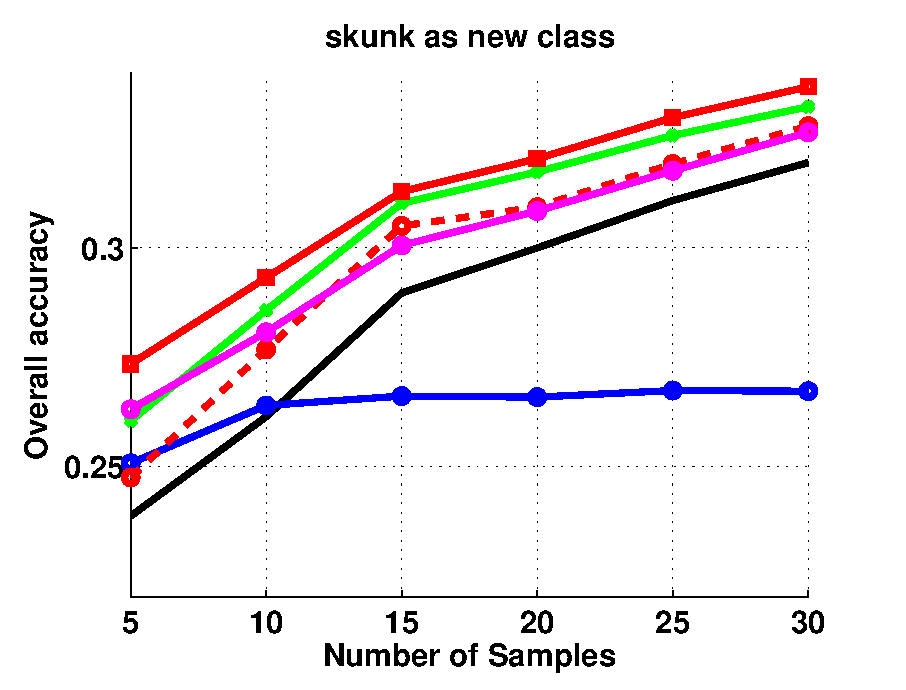
\includegraphics[width=0.18\textwidth]{fig/A2A_bad/A2A_bad_3c_9.eps}  }
  \subfloat[]{    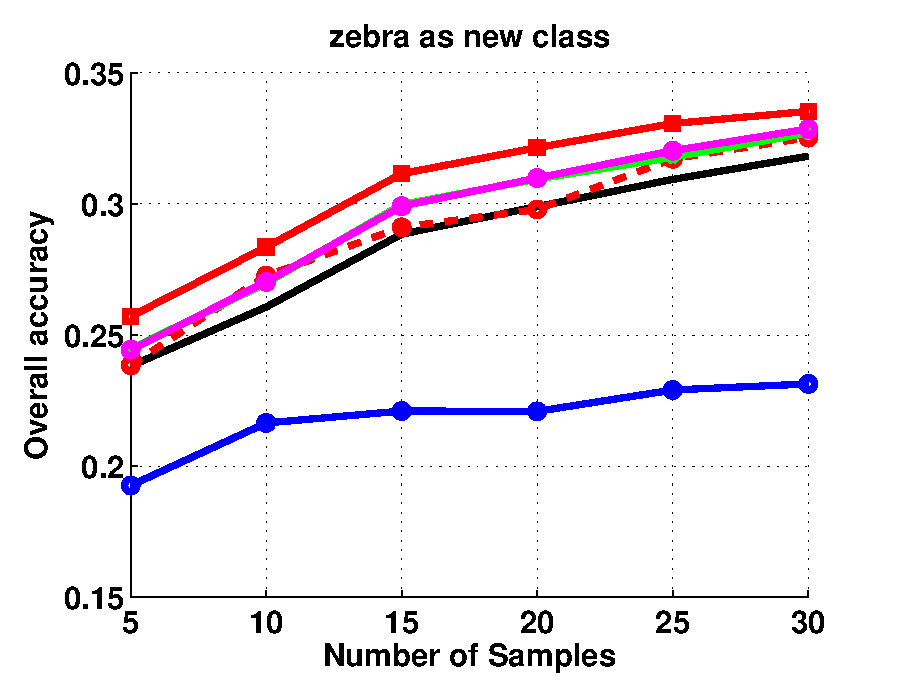
\includegraphics[width=0.18\textwidth]{fig/A2A_bad/A2A_bad_3c_10.eps}  }\\
  \caption{A2A bad, 3 classes }\label{fig:a2a_bad_3}
\end{figure*}
\begin{figure*}
  \centering
  \subfloat[]{    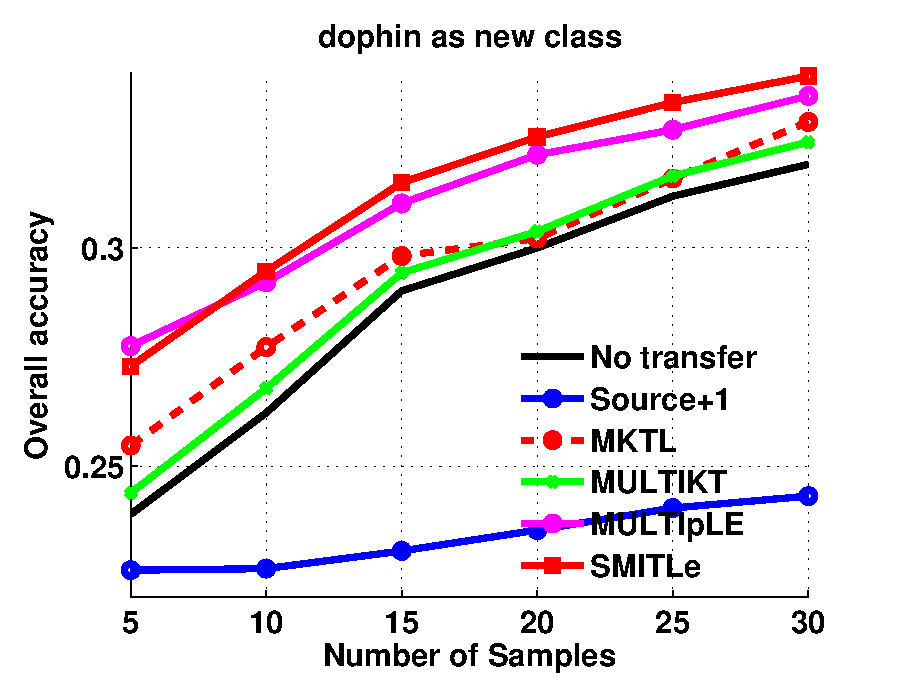
\includegraphics[width=0.18\textwidth]{fig/A2A_bad/A2A_bad3.eps}  }
  \subfloat[]{    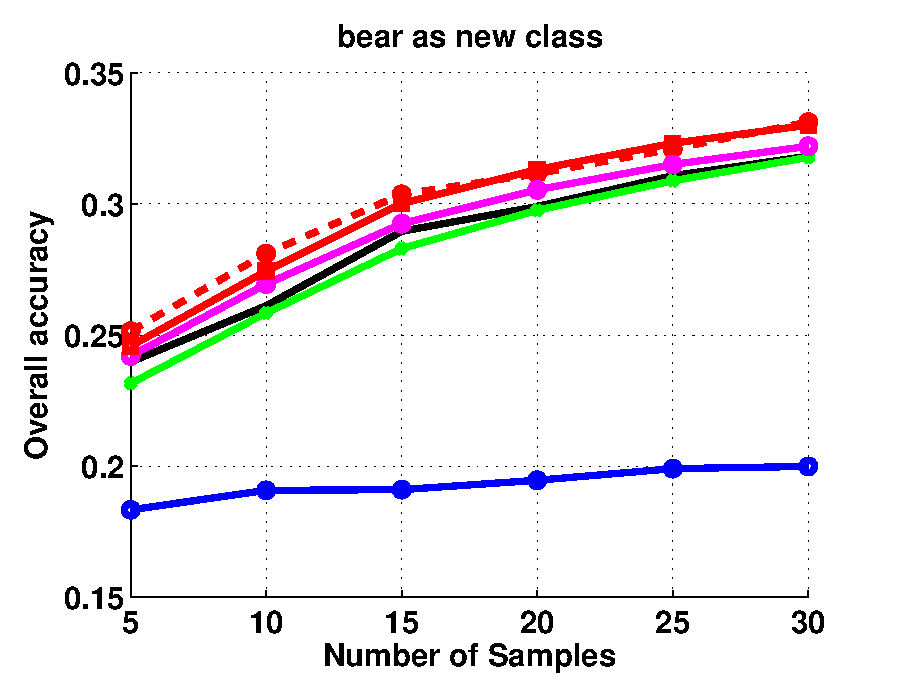
\includegraphics[width=0.18\textwidth]{fig/A2A_bad/A2A_bad2.eps}  }
  \subfloat[]{    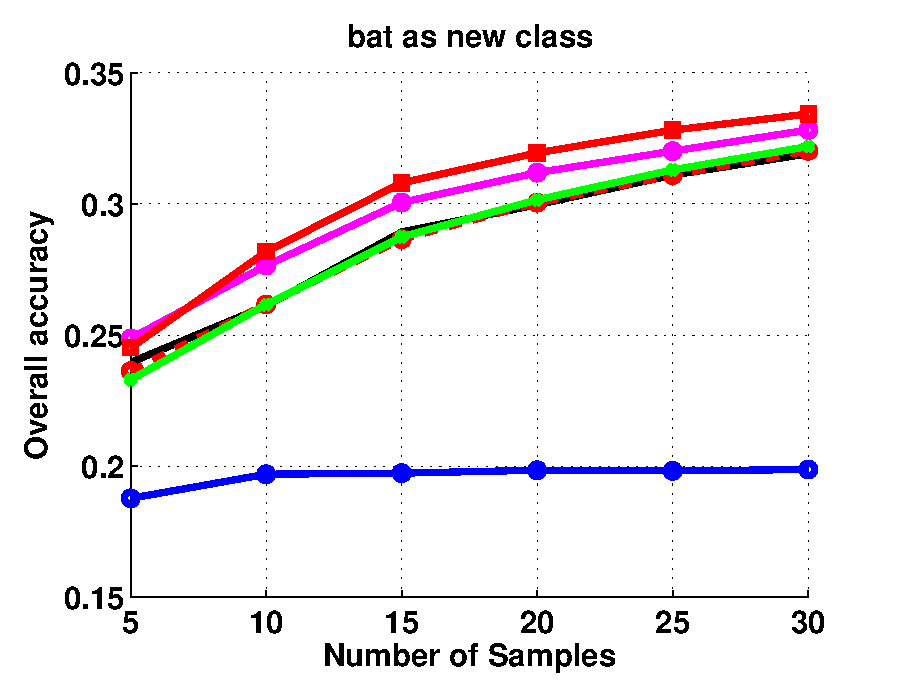
\includegraphics[width=0.18\textwidth]{fig/A2A_bad/A2A_bad1.eps}  }
  \subfloat[]{    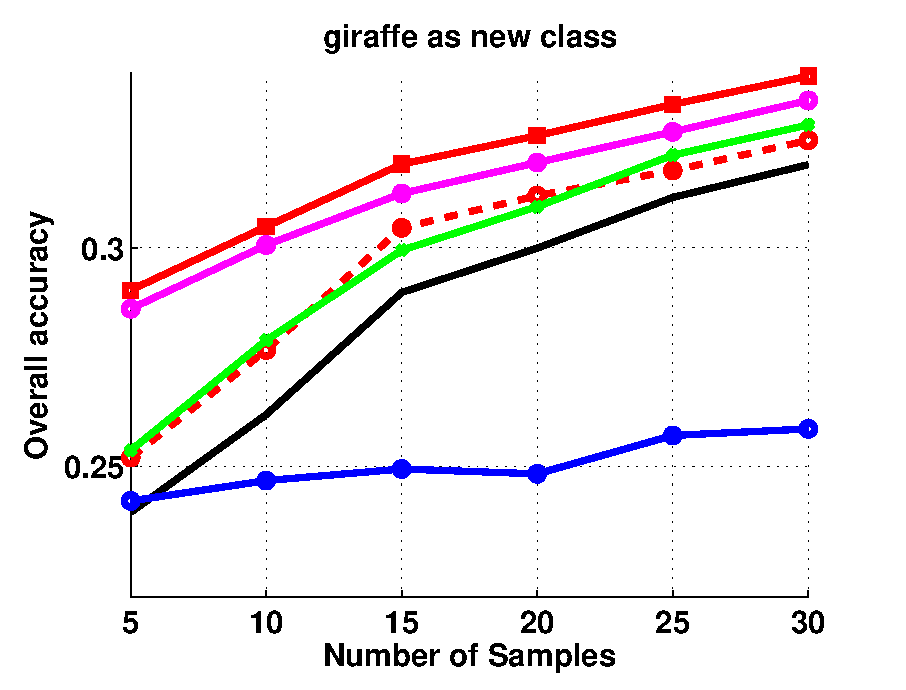
\includegraphics[width=0.18\textwidth]{fig/A2A_bad/A2A_bad4.eps}  }
  \subfloat[]{    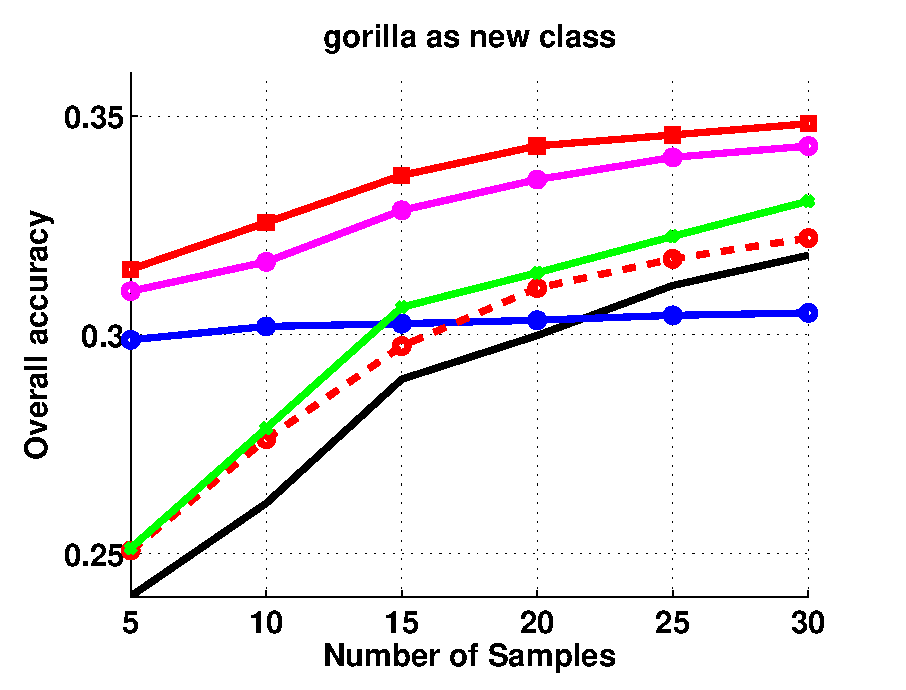
\includegraphics[width=0.18\textwidth]{fig/A2A_bad/A2A_bad5.eps}  }\\
  \subfloat[]{    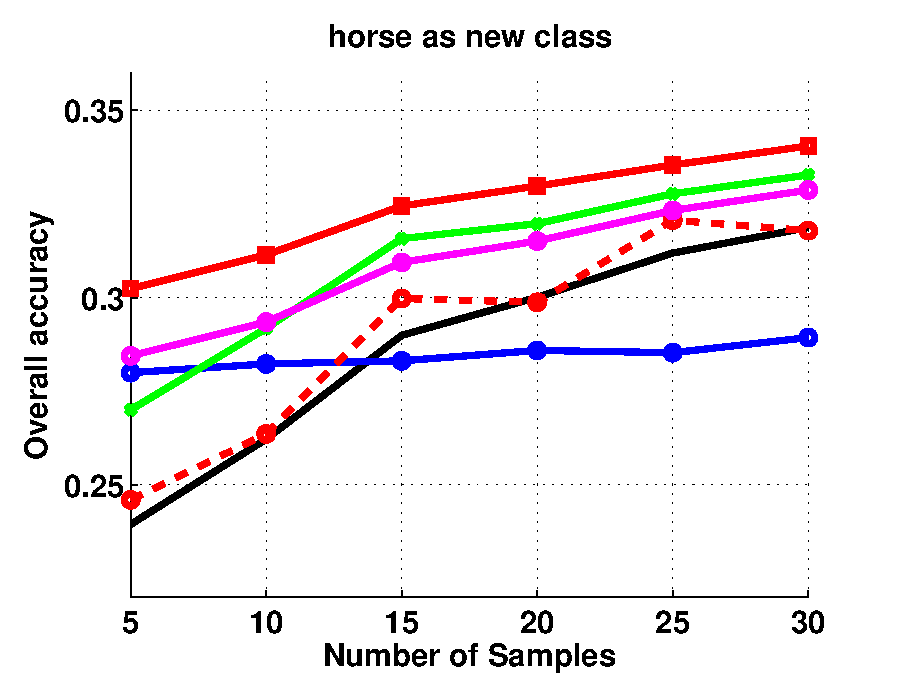
\includegraphics[width=0.18\textwidth]{fig/A2A_bad/A2A_bad6.eps}  }
  \subfloat[]{    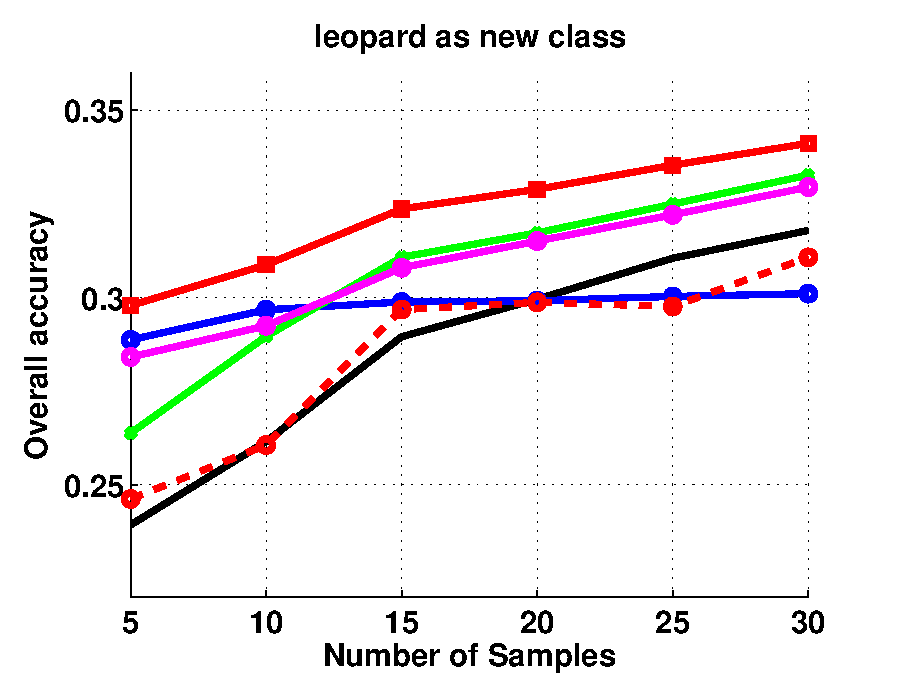
\includegraphics[width=0.18\textwidth]{fig/A2A_bad/A2A_bad7.eps}  }
  \subfloat[]{    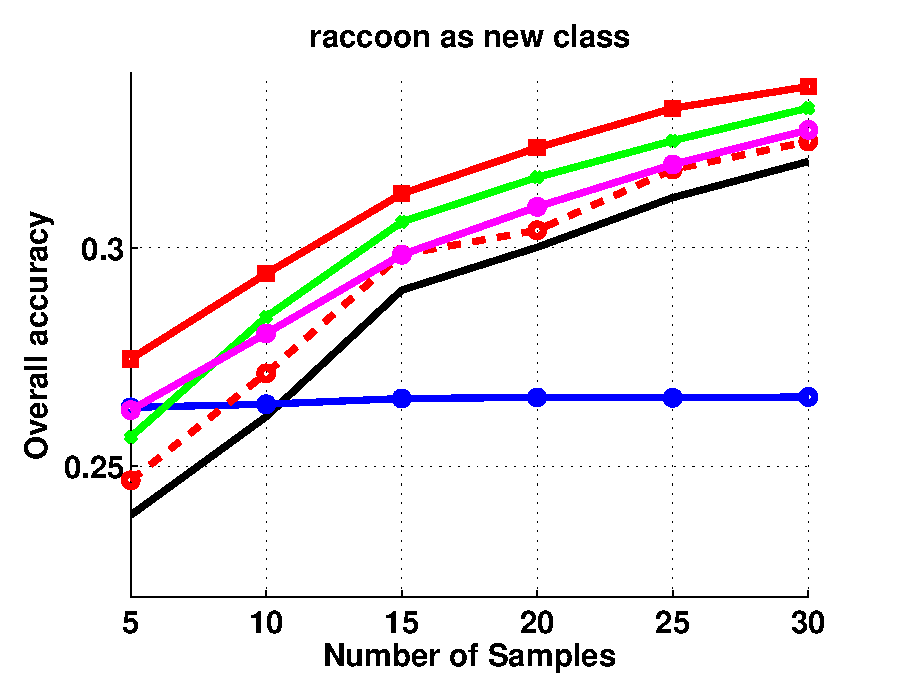
\includegraphics[width=0.18\textwidth]{fig/A2A_bad/A2A_bad8.eps}  }
  \subfloat[]{    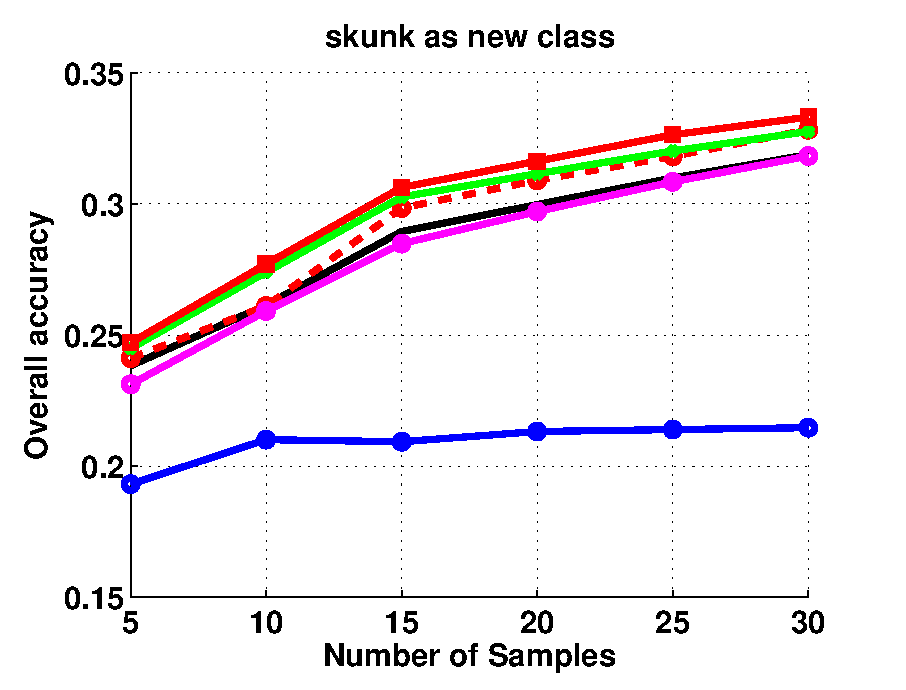
\includegraphics[width=0.18\textwidth]{fig/A2A_bad/A2A_bad9.eps}  }
  \subfloat[]{    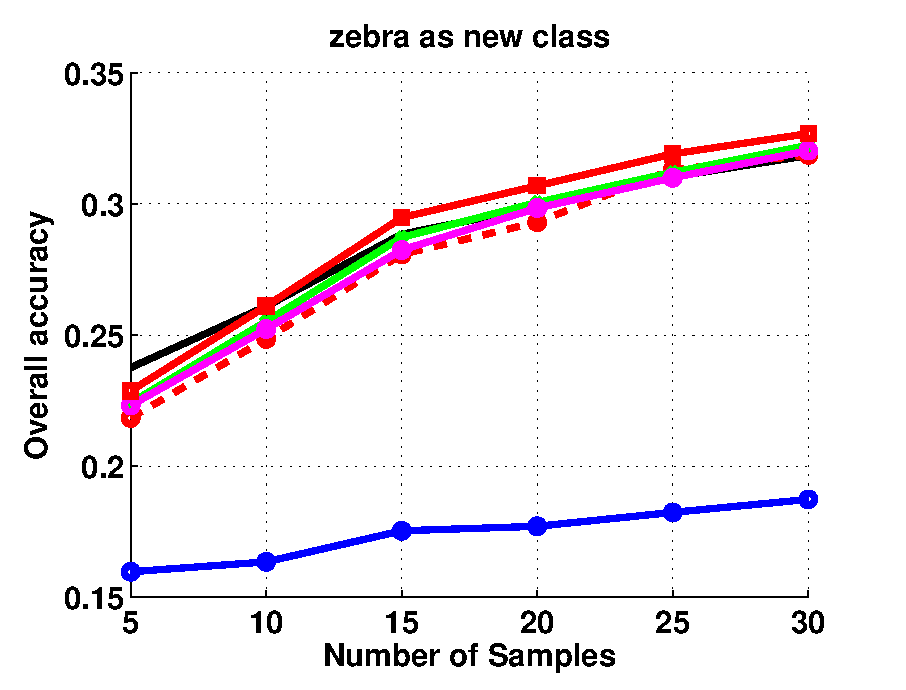
\includegraphics[width=0.18\textwidth]{fig/A2A_bad/A2A_bad10.eps}  }\\
  \caption{A2A bad, 4 classes }\label{fig:a2a_bad_4}
\end{figure*}